%!TEX root = ../thesis-main.tex
\chapter{Tecnologie e Progettazione}
\label{chap:technologies}

Questo capitolo presenta l'analisi degli obiettivi e la progettazione del sistema EcoSpot, descrivendo l'architettura logica e le scelte tecnologiche adottate per lo sviluppo dell'applicazione mobile e la sua integrazione con i servizi cloud e IoT.


\section{Obiettivi del progetto}
\label{sec:project_goals}

La progettazione di EcoSpot è guidata da quattro obiettivi strategici, volti a coniugare l'esperienza turistica con la consapevolezza ecologica e le moderne tecnologie mobili.

\begin{itemize}
    \item \textbf{Divulgazione e Citizen Science:} l'obiettivo è diffondere la conoscenza della biodiversità locale attraverso una \textit{collezione digitale} strutturata e partecipativa. L'applicazione non si limita a offrire un catalogo dettagliato di specie (suddivise in categorie come uccelli, mammiferi, pesci e aree verdi), ma abilita pratiche di \textit{Citizen Science}: gli utenti possono contribuire attivamente al monitoraggio del territorio inviando segnalazioni georeferenziate e fotografiche, trasformando la semplice osservazione in un percorso di tutela condivisa.

    \item \textbf{Incentivazione del turismo lento:} il sistema mira a favorire un'esplorazione rispettosa del territorio sfruttando meccaniche \textit{location-based}. Grazie alla geolocalizzazione e al \textit{geofencing}, l'utente è incentivato a raggiungere fisicamente luoghi reali (valli, argini, punti di osservazione) per sbloccare i contenuti e validare le scoperte, promuovendo così una mobilità dolce e un presidio attivo degli habitat, in contrapposizione al turismo di massa.

    \item \textbf{Monitoraggio ambientale integrato:} il progetto intende rendere accessibili parametri ecologici complessi tramite l'aggregazione di dati IoT in tempo reale. L'app si interfaccia con le API di enti territoriali (es. progetto DISCOV.ER) per i dati idrografici (livello, temperatura, conducibilità) e integra servizi meteorologici come Open-Meteo \cite{open_meteo_api}, rendendo visibili all'utente fattori invisibili ma vitali per l'ecosistema lagunare.

    \item \textbf{Incremento del coinvolgimento (Gamification):} l'ultimo obiettivo è massimizzare la ritenzione e la partecipazione dell'utente attraverso la \textit{gamification}. L'uso di elementi ludici come punti esperienza (XP) e livelli dinamici (da ``Esploratore'' a ``Leggenda del Delta'') serve a rafforzare il senso di appartenenza al territorio e a stimolare comportamenti virtuosi, premiando l'interazione fisica con il Parco.
\end{itemize}

L'integrazione di questi quattro pilastri mira ad aumentare l'attenzione dei visitatori, offrendo un'esperienza che combina contenuti informativi, esplorazione fisica e feedback immediati sulle pratiche sostenibili. Al tempo stesso, la possibilità di accedere a dati ambientali in tempo quasi reale e di collegarli alle osservazioni sul campo contribuisce a sviluppare una maggiore consapevolezza ecologica, mostrando in modo concreto la fragilità e il valore degli ecosistemi lagunari. In questo senso, EcoSpot si configura non solo come strumento di guida turistica, ma come piattaforma di educazione ambientale e di supporto alla gestione sostenibile delle aree protette del Delta del Po.

\section{Analisi dei Requisiti}
\label{sec:requirements}

La fase di progettazione è stata preceduta da un'analisi dettagliata dei requisiti, volta a definire il perimetro funzionale e le caratteristiche qualitative del sistema EcoSpot.

\subsection{Requisiti Funzionali}
I requisiti funzionali descrivono le interazioni specifiche tra l'utente e il sistema e definiscono le necessità informative della base di dati. Sulla base degli obiettivi di progetto e dei casi d'uso identificati, sono stati definiti i seguenti requisiti:

\begin{enumerate}
    \item \textbf{Mappa Interattiva} \label{req:mappa}
    Il sistema deve fornire una mappa digitale del Delta del Po che visualizzi i layer informativi relativi alle aree di interesse naturalistico (flora e fauna) e alle stazioni di monitoraggio ambientale. La mappa deve supportare l'interazione touch (pan e zoom) e adattare la densità delle informazioni in base al livello di zoom.

    \item \textbf{Posizione in Tempo Reale} \label{req:tracking}
    L'applicazione deve acquisire e monitorare costantemente la posizione geografica dell'utente tramite GPS. Il tracciamento deve avvenire in background (ove permesso) o in foreground per garantire che la posizione sulla mappa sia sempre sincronizzata con lo spostamento fisico dell'utente.
    
    \item \textbf{Rilevamento di Prossimità} \label{req:geofencing}
    Per supportare la meccanica del "Turismo Lento", il sistema deve calcolare in tempo reale la distanza euclidea tra le 
    coordinate dell'utente e gli habitat o le aree verdi. Al raggiungimento di una soglia di tolleranza 
    specifica (definita come \textit{raggio di scoperta}, variabile tra 450 metri per la fauna e 800 metri per la flora), 
    il sistema deve innescare l'evento di "scoperta".
    
    \item \textbf{Profilo Utente} \label{req:profilo}
    Il database deve mantenere un profilo utente persistente e sincronizzato su cloud per gli utenti registrati, 
    memorizzando dati anagrafici e preferenze. Il sistema deve altresì supportare una modalità \enquote{Ospite} con persistenza 
    locale temporanea.
    
    \item \textbf{Sistema di Gamification} \label{req:gamification}
    Il sistema deve gestire la logica di progressione dell'utente. Ogni evento di scoperta deve assegnare una ricompensa in Punti Esperienza (XP), aggiornare l'inventario delle specie collezionate (sbloccando le relative schede informative) e ricalcolare il rango e il livello utente in base alle soglie predefinite.

    \item \textbf{Ricerca} \label{req:ricerca}
    Data l'elevata densità di elementi sulla mappa, il sistema deve fornire una barra di ricerca testuale per le specie e le aree verdi. 
    Questi strumenti devono permettere all'utente di ridurre la complessità visiva e isolare rapidamente i dati di interesse.

    \item \textbf{Dati Ambientali} \label{req:iot}
    Il sistema deve ingerire e visualizzare dati provenienti da fonti esterne eterogenee (stazioni \ac{IoT}). Il modello dati deve prevedere strutture flessibili per normalizzare letture di temperatura, livello idrometrico e conducibilità, rendendole consultabili in tempo quasi reale attraverso i marker sulla mappa.

    \item \textbf{Segnalazione} \label{req:segnalazioni}
    Gli utenti autenticati devono poter inviare segnalazioni georeferenziate. Ogni record deve comprendere una descrizione 
    testuale, la posizione GPS esatta (\texttt{GeoPoint}) e il timestamp di creazione. Le prove fotografiche devono essere 
    caricate su uno storage remoto (\textit{Cloud Storage}).

    \item \textbf{Progressione} \label{req:integrita}
    Per incentivare l'uso continuativo e garantire la coerenza dei dati, ogni modifica allo stato del giocatore (scoperta, level-up) deve essere gestita tramite transazioni atomiche. Questo impedisce condizioni di gara (race conditions) e duplicazioni di XP, assicurando che l'aggiornamento del livello e dell'inventario avvengano come un'operazione indivisibile.

    \item \textbf{Funzionamento Offline e Sincronizzazione} \label{req:offline}
    Considerata la potenziale assenza di copertura di rete in alcune aree del parco, il sistema deve garantire la fruibilità dei contenuti statici (schede informative) e della mappa (tramite caching) anche in modalità offline. Le azioni critiche dell'utente, come lo sblocco di una specie o l'invio di una segnalazione, devono essere memorizzate localmente in una coda di persistenza e sincronizzate automaticamente con il server remoto non appena la connettività viene ripristinata.

    \item \textbf{Compatibilità Multi-Piattaforma} \label{req:multipiattaforma}
    Il sistema deve essere sviluppato garantendo la piena compatibilità funzionale e visiva sia con il sistema operativo 
    Android che con iOS. L'interfaccia utente deve adattarsi alle linee guida specifiche delle piattaforme pur mantenendo un 
    design system coerente (Material Design 3) \cite{material_design_3}.
\end{enumerate}
\subsection{Requisiti Non Funzionali}
I requisiti non funzionali definiscono gli attributi di qualità del sistema, imponendo vincoli architetturali e prestazionali 
necessari per garantire un'esperienza utente soddisfacente, specialmente in un contesto di utilizzo in mobilità e all'aperto.

\begin{enumerate}
    \item \textbf{Usabilità e Accessibilità} \label{rnf:usabilita}
    L'interfaccia utente deve garantire la massima leggibilità anche in condizioni di forte illuminazione solare diretta, 
    tipica delle escursioni diurne. Il sistema deve supportare il passaggio dinamico (o automatico) tra tema chiaro e scuro 
    per mantenere un contrasto ottimale.

    \item \textbf{Prestazioni e Reattività} \label{rnf:performance}
    Il rendering della mappa e delle animazioni di transizione deve mantenere un frame rate stabile per evitare scatti (\textit{jank}) che comprometterebbero l'esperienza utente. Il tempo di avvio dell'applicazione (Cold Start) non deve superare i 2 secondi su dispositivi di fascia media.

    \item \textbf{Efficienza Energetica} \label{rnf:energia}
    Dato l'uso prolungato durante le escursioni e l'assenza di punti di ricarica nelle aree naturali, il consumo della batteria deve essere minimizzato. Il servizio di localizzazione deve adottare strategie di campionamento adattivo (es. riducendo la frequenza di aggiornamento GPS quando l'utente è fermo) per non drenare eccessivamente le risorse del dispositivo.

    \item \textbf{Manutenibilità del Codice} \label{rnf:manutenibilita}
    Il codice sorgente deve seguire i principi della \textit{Clean Architecture}, garantendo una netta separazione tra logica di business, interfaccia utente e gestione dei dati. L'adozione di standard di formattazione coerenti e la documentazione del codice devono facilitare le operazioni di debug e l'aggiornamento futuro del software da parte di altri sviluppatori.

    \item \textbf{Estensibilità e Scalabilità} \label{rnf:estensibilita}
    L'architettura del sistema deve essere progettata per accogliere future evoluzioni senza richiedere la riscrittura dei moduli principali. Deve essere possibile aggiungere nuove categorie di specie, nuovi layer cartografici o funzionalità di gamification aggiuntive (es. classifiche globali) attraverso l'estensione delle classi esistenti o l'integrazione di nuovi plugin.

\end{enumerate}
\section{Tecnologie}
\label{sec:technologies}

\subsection{Flutter e Dart}
L'applicazione EcoSpot è sviluppata con \textbf{Flutter} \cite{flutter}, il framework open-source di Google che consente la realizzazione di applicazioni multipiattaforma native.
L'adozione di questa architettura risponde agli obiettivi del progetto garantendo:

\begin{itemize}
    \item \textbf{Efficienza nello sviluppo (Single Codebase):} Flutter permette di gestire un'unica base di codice per Android e iOS. Questo approccio riduce i tempi di implementazione e assicura una parità di funzionalità tra le piattaforme (Requisito \ref{req:multipiattaforma}).

    \item \textbf{Prestazioni grafiche (Impeller):} Il sistema sfrutta il motore di rendering \textbf{Impeller}, che sostituisce il precedente Skia. Impeller risolve i problemi di \textit{jank} (scatti) pre-compilando gli shader e sfruttando le API di basso livello (Metal su iOS e Vulkan su Android). Ciò garantisce animazioni fluide a 60 FPS, fondamentali per la gestione delle mappe interattive (Requisito \ref{rnf:performance}).

    \item \textbf{Produttività (Hot Reload):} La funzionalità di \textit{Stateful Hot Reload} consente l'iniezione delle modifiche al codice in tempo reale, ottimizzando il ciclo di raffinamento dell'interfaccia utente (UI).

    \item \textbf{Ecosistema e Modularità:} L'architettura integra pacchetti maturi come \texttt{flutter\_map} per la cartografia, \texttt{geolocator} per il tracciamento GPS e \texttt{riverpod} per la gestione dello stato.
\end{itemize}

Il linguaggio alla base del framework è \textbf{Dart}, caratterizzato da una duplice natura: ottimizzato per la UI e fortemente orientato alla programmazione asincrona.
In particolare, il supporto nativo per \texttt{Future} e \texttt{Stream} (Requisito \ref{req:tracking}) semplifica notevolmente la gestione dei flussi di dati in tempo reale di EcoSpot, come l'aggiornamento della posizione dell'utente e il recupero dei dati dai sensori IoT, permettendo l'esecuzione di task complessi senza bloccare il thread principale dell'interfaccia.

Nel contesto del progetto, l'utilizzo di Flutter e Dart offre una soluzione scalabile, capace di sostenere i requisiti di gamification e citizen science con un'esperienza utente di livello nativo.
\subsection{Backend, Servizi Cloud e API}
L'infrastruttura di backend gestisce i dati e la persistenza delle informazioni, garantendo sincronizzazione in tempo reale, 
sicurezza e disponibilità del servizio. Le tecnologie adottate rispondono a criteri di scalabilità, ridotta manutenzione 
infrastrutturale (approccio \textit{Serverless}) e facilità di integrazione con l'ecosistema mobile.
Le principali componenti progettuali includono:

\begin{itemize}
    \item \textbf{Architettura Serverless e Cloud Services:} A differenza delle architetture tradizionali, il sistema non utilizza un server monolitico proprietario ma si appoggia alla suite \textbf{Google Firebase} come Backend-as-a-Service (BaaS). Questo approccio delega la complessità della gestione server, permettendo all'applicazione di interagire direttamente con i servizi cloud tramite SDK nativi sicuri, garantendo alte prestazioni e riducendo i tempi di latenza.

    \item \textbf{Database NoSQL:} Il sistema utilizza \texttt{Cloud Firestore}, un database orientato ai documenti che 
    consente all'app mobile di sincronizzare i dati in tempo reale tra i dispositivi. A differenza dei database relazionali, 
    Firestore offre una struttura flessibile organizzata in collezioni 
    (es. \texttt{users}, \texttt{reports}, \texttt{species}), ottimizzata per letture frequenti e funzionamento offline. 
    La persistenza locale permette agli utenti di consultare i dati e salvare progressi anche in assenza di connettività (Requisito \ref{req:offline}), 
    con sincronizzazione automatica al ripristino della rete.

    \item \textbf{Gestione della Logica e dello Stato (Controller):} La logica applicativa lato client e il flusso dei dati sono gestiti attraverso il framework \textbf{Riverpod}. I provider agiscono come controller intelligenti che orchestrano le operazioni asincrone: mediano le richieste tra l'interfaccia utente (UI) e i repository dei dati, aggiornando dinamicamente le viste senza bloccare il thread principale.

    \item \textbf{Autenticazione e Sicurezza:} Il modulo \texttt{Firebase Authentication} gestisce l'identità degli utenti, 
    supportando un sistema ibrido che include l'accesso anonimo e l'autenticazione federata tramite terze parti come Google (Requisito \ref{req:profilo}). 
    Questo componente assicura che le operazioni di scrittura sul database 
    (come l'invio di segnalazioni o l'aggiornamento dei livelli) siano consentite solo a utenti validati, 
    proteggendo i dati sensibili attraverso regole di sicurezza lato server.

    \item \textbf{Elaborazione Gamification e Citizen Science:} Le attività di monitoraggio e le meccaniche di gioco sono processate attraverso una logica distribuita. Il client mobile calcola in tempo reale le interazioni spaziali (distanza dai POI tramite GPS), mentre il backend si occupa della validazione e dello storage delle segnalazioni fotografiche (\textit{Citizen Science}) tramite \texttt{Cloud Storage}, garantendo l'integrità del percorso di crescita dell'utente (XP e livelli).

    \item \textbf{Integrazione con API Esterne e IoT:} Il sistema è progettato per comunicare con servizi di terze parti per arricchire il contesto ambientale. L'applicazione consuma le API di \texttt{Open-Meteo} per i dati climatici e si interfaccia con endpoint dedicati per il recupero dei dati dai sensori \ac{IoT}, 
    normalizzando formati eterogenei in un'unica esperienza utente coerente (Requisito \ref{req:iot}).
\end{itemize}

Questa architettura modulare consente di mantenere separati i livelli di presentazione (Widget Flutter), gestione dello stato (Riverpod) e servizi dati (Firebase/API), favorendo la manutenibilità del codice e la possibilità di estendere le funzionalità senza impattare sulla stabilità del sistema esistente.

\subsection{Riverpod}
Per garantire la scalabilità e la manutenibilità di un ecosistema complesso come \textbf{EcoSpot}, l'architettura software si fonda su \textbf{Riverpod}, un framework di \textit{Reactive Caching} e \textit{Dependency Injection}. Questo strumento non si limita alla semplice gestione dello stato, ma agisce come il sistema nervoso dell'applicazione, orchestrando in modo dichiarativo e sicuro il flusso di dati eterogenei dai servizi Firebase alle API REST, fino ai sensori GPS che convergono nell'applicazione.

L'adozione di Riverpod ha permesso in primo luogo di disaccoppiare nettamente l'interfaccia utente dalla logica di business: i widget, come la mappa interattiva (\texttt{MapWidget}) o le schede di dettaglio, non contengono logica imperativa di recupero dati, ma si limitano a ``osservare'' passivamente lo stato fornito dai provider tramite il metodo \texttt{ref.watch}. Questa separazione delle responsabilità rende il codice modulare, facilitando notevolmente le operazioni di testing e la manutenzione evolutiva del software.

Un vantaggio cruciale dell'architettura risiede nella gestione unificata dell'asincronicità. Il progetto deve armonizzare sorgenti dati con nature temporali opposte, gestendo simultaneamente flussi in tempo reale, come la posizione GPS o lo stato di autenticazione, e chiamate asincrone puntuali, come il recupero dei dati meteo o dei sensori IoT. Riverpod astrae questa complessità gestendo automaticamente gli stati di caricamento, errore e successo, garantendo che l'interfaccia utente non si blocchi mai e possa reagire istantaneamente ai cambiamenti, come l'aggiornamento automatico della mappa al variare della posizione dell'utente.

Tale reattività è potenziata da un meccanismo di \textit{Dependency Injection} dichiarativa, che consente ai provider di dipendere l'uno dall'altro per generare stati derivati. Un esempio chiave nel progetto è rappresentato dallo \texttt{speciesProvider}: esso combina i dati statici delle specie con il profilo dinamico dell'utente, ricalcolando automaticamente quali specie segnare come ``visitate'' ogni volta che avviene una nuova scoperta. Questo approccio propaga l'aggiornamento a tutta l'applicazione senza la necessità di callback complessi o gestione manuale degli stati.
Infine, a differenza di altre soluzioni, Riverpod garantisce una sicurezza ``Compile-safe'', eliminando a tempo di compilazione errori comuni come il \texttt{ProviderNotFoundException} e assicurando che ogni componente abbia sempre accesso alle dipendenze necessarie, come \texttt{AuthService} o \texttt{DatabaseHelper}, in modo tipizzato e robusto.
\subsection{Integrazione di Servizi e Fonti Dati}
Per raggiungere gli obiettivi di sensibilizzazione ambientale e gamification, EcoSpot non opera come un sistema isolato, ma agisce come collettore di dati provenienti da fonti eterogenee. L'architettura è stata progettata per integrare servizi di terze parti che arricchiscono l'esperienza utente con informazioni contestuali in tempo reale.
\begin{itemize}
    \item \textbf{Monitoraggio Ambientale e Consapevolezza}: l'integrazione con le reti di sensori IoT risponde all'esigenza educativa di rendere visibili parametri ecologici (come livello idrometrico e salinità) altrimenti invisibili al turista. La scelta di utilizzare dati reali serve a creare un collegamento diretto tra le condizioni chimico-fisiche dell'habitat e la biodiversità osservata, trasformando l'applicazione in uno strumento di divulgazione scientifica attiva.
    \item \textbf{Geolocalizzazione e Cartografia Open Source}: la componente cartografica si basa sulla piattaforma 
    \textbf{OpenStreetMap}. Questa soluzione garantisce la flessibilità necessaria per rappresentare sentieri e aree naturali spesso assenti nelle mappe commerciali.
    \item \textbf{Contestualizzazione Meteorologica}: le condizioni atmosferiche influenzano l'etologia delle specie e la fruibilità del parco. Il sistema integra servizi meteorologici esterni (come \textbf{Open-Meteo}) per fornire all'utente un quadro immediato delle condizioni ambientali. Questo dato non è puramente informativo, ma arricchisce le segnalazioni di \textit{Citizen Science}, permettendo di correlare gli avvistamenti faunistici con le variabili climatiche del momento.
\end{itemize}

\section{Architettura del Sistema}
\label{sec:system_architecture}

Dati i requisiti funzionali precedentemente definiti, è possibile delineare l'architettura logica del sistema EcoSpot. La struttura è concepita come un ecosistema modulare composto da quattro componenti principali, che collaborano per garantire un'esperienza utente reattiva e scalabile.

L'esperienza dell'utente è mediata interamente dallo \textit{smartphone}, che agisce sia come portale d'accesso ai contenuti sia come strumento di controllo delle funzionalità. L'applicazione integra \textbf{OpenStreetMap}, una piattaforma cartografica libera che fornisce dati geografici dettagliati e costantemente aggiornati da una comunità globale. 
A differenza delle soluzioni proprietarie, l'integrazione di OpenStreetMap (tramite il motore di rendering \texttt{flutter\_map}) 
consente una personalizzazione avanzata della visualizzazione delle aree naturali del Delta, permettendo all'utente di 
orientarsi e navigare in tempo reale verso i punti di interesse (POI) disseminati nel territorio (Requisito \ref{req:mappa}).

Il cuore della gestione dei dati è affidato a \textbf{Google Cloud Firestore}. Questo database NoSQL orientato ai documenti è utilizzato per memorizzare in modo strutturato tutte le informazioni vitali del sistema: dai profili utente ai progressi di gioco (livelli e XP), fino all'inventario delle specie scoperte (i dettagli sulla struttura dati sono approfonditi nella Sezione \ref{sec:data_modeling}). La scelta di utilizzare una soluzione cloud-based, supportata da \textbf{Cloud Storage} per l'archiviazione delle immagini fotografiche, risponde all'esigenza di centralizzare i contributi di \textit{Citizen Science}, rendendo le segnalazioni immediatamente sicure e accessibili per future analisi, garantendo al contempo la sincronizzazione dei dati tra diversi dispositivi dello stesso utente (si veda Sezione \ref{sec:citizen_science}).

Per la gestione delle logiche spaziali, il sistema sfrutta la potenza di calcolo locale del dispositivo attraverso il 
pacchetto \textbf{Geolocator}. Invece di dipendere costantemente dal server per ogni verifica, l'applicazione calcola 
direttamente sul client le distanze 
euclidee tra la posizione dell'utente e gli habitat. Questo approccio decentralizzato permette di validare le scoperte 
(meccanismo di \textit{geofencing}) in tempo reale (Requisito \ref{req:geofencing}) e con latenza zero, riducendo il consumo di dati mobili e migliorando 
l'esperienza anche in aree con scarsa copertura di rete.

Infine, per contestualizzare l'esperienza nell'ambiente reale, il sistema agisce come un aggregatore di dati esterni tramite 
protocolli \textbf{HTTP/REST}. L'applicazione interroga periodicamente le API di servizi terzi, come le stazioni di 
monitoraggio \ac{IoT} 
per i livelli idrometrici e il servizio \textbf{Open-Meteo} per le condizioni atmosferiche. Questa integrazione assicura 
che le informazioni mostrate all'utente non siano solo statiche, ma riflettano le condizioni dinamiche e vitali 
dell'ecosistema lagunare al momento della visita (Requisito \ref{req:iot}).

\begin{figure}[htbp]
    \centering
    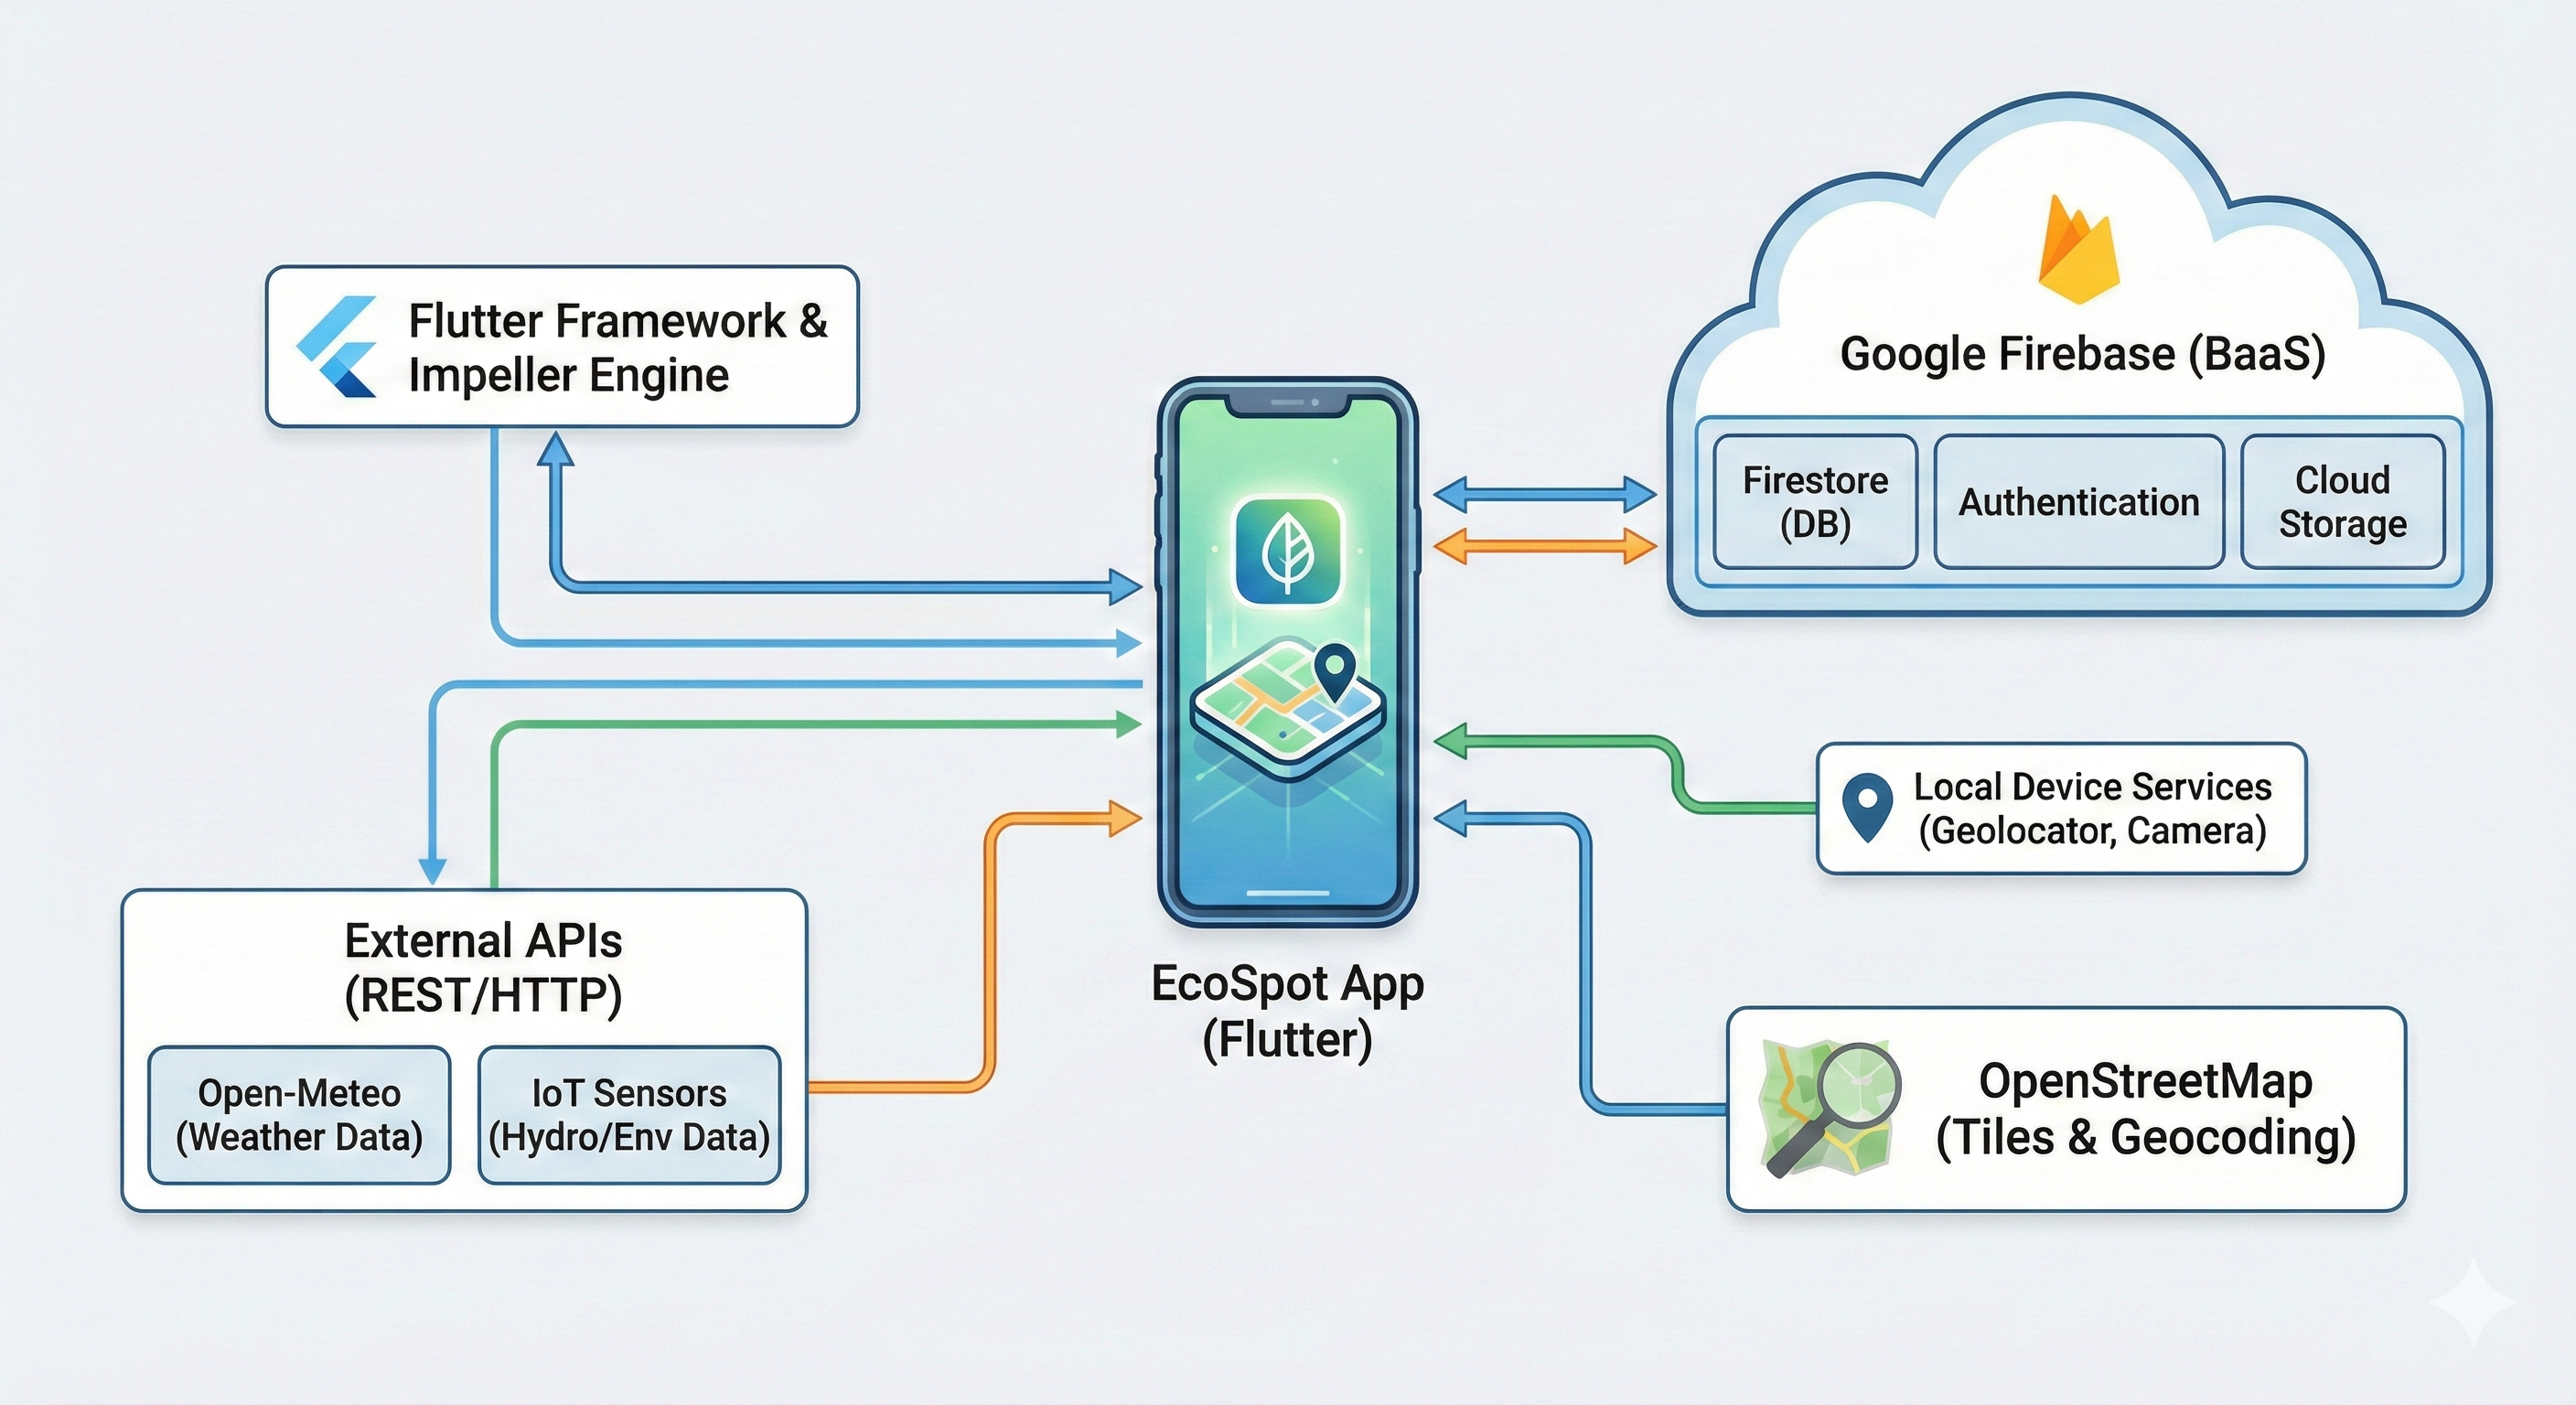
\includegraphics[width=0.9\textwidth]{figures/schema/architecture_schema.png}
    
    \caption[Schema Architetturale di EcoSpot]{Schema logico dell'architettura di sistema.}
    
    \label{fig:system_architecture_schema}
\end{figure}
\section{User Experience}
\label{sec:ux_design}

La progettazione dell'interfaccia utente (UI) di EcoSpot risponde a precise esigenze ergonomiche e comunicative legate al contesto outdoor, adottando le linee guida del \textit{Material Design 3} per garantire coerenza e accessibilità.

\subsection{Palette cromatica}
La palette cromatica di EcoSpot crea un legame visivo diretto con l'ambiente del Delta del Po. Il colore primario, 
una tonalità di verde desaturato, \textbf{si ispira} all'identità visiva del progetto \textit{DISCOV.ER} (Digital Twin and Citizen Science for the Sustainability of Areas of Natural and Tourist Interest)
\cite{discover_project} e richiama la vegetazione alofila tipica delle aree lagunari, trasmettendo un senso di continuità 
tra l'interfaccia digitale e l'ecosistema circostante.

Questa specifica tonalità di verde desaturato è stata scelta per richiamare la vegetazione alofila e le praterie sommerse tipiche delle aree lagunari, con l'obiettivo di trasmettere all'utente un senso di continuità tra l'interfaccia digitale e l'ecosistema circostante. 

Un aspetto centrale della progettazione rimane l'uso semantico del colore per indicare la \textbf{rarità delle specie}, facilitando una valutazione istantanea del valore di un avvistamento sulla mappa:
\begin{itemize}
    \item \textbf{Grigio:} Specie Comuni (\texttt{rarityCommon}).
    \item \textbf{Verde:} Specie Non Comuni (\texttt{rarityUncommon}).
    \item \textbf{Blu:} Specie Rare (\texttt{rarityRare}).
    \item \textbf{Viola:} Specie Epiche (\texttt{rarityEpic}).
    \item \textbf{Oro:} Specie Leggendarie (\texttt{rarityLegendary}).
\end{itemize}
Questa codifica visiva permette all'utente di valutare istantaneamente il valore di una scoperta durante la navigazione sulla mappa.

\subsection{Temi Adattivi}
Al fine di assicurare un'esperienza visiva ottimale in qualsiasi condizione ambientale, l'applicazione implementa un sistema 
di \textbf{Temi Adattivi}, rispondendo puntualmente al requisito di usabilità (Requisito \ref{rnf:usabilita}). 
Il sistema è in grado di rilevare le preferenze del dispositivo e commutare automaticamente tra due configurazioni cromatiche 
distinte: la \textbf{Light Mode}, caratterizzata da sfondi chiari e testi ad alto contrasto per garantire la leggibilità 
sotto la luce solare diretta, e la \textbf{Dark Mode}. Quest'ultima adotta sfondi scuri progettati per ridurre 
l'affaticamento visivo e il consumo energetico sui display OLED, minimizzando al contempo l'impatto luminoso sulla fauna 
durante le osservazioni nelle ore crepuscolari. L'utente mantiene comunque il controllo completo sull'interfaccia, potendo 
forzare manualmente la modalità desiderata tramite l'area impostazioni, con la garanzia che tale preferenza venga memorizzata 
e sincronizzata in cloud tramite il profilo Firebase.

\subsection{Pattern di Navigazione}
La navigazione è stata progettata per minimizzare il carico cognitivo attraverso una struttura ibrida.

La \textbf{Bottom Navigation Bar} costituisce il punto di accesso principale per le macro-aree dell'applicazione 
(\textit{Esplora}, \textit{Statistiche} e \textit{Impostazioni}), garantendo una transizione rapida tra la mappa e l'area 
di gestione del profilo. La barra utilizza indicatori visivi e colori semantici per evidenziare la sezione attiva, riducendo 
lo sforzo mnemonico dell'utente.
Per la visualizzazione dei dettagli di specie, aree verdi e stazioni di monitoraggio, si è scelto di utilizzare i \textbf{Modal Bottom Sheets} che coprono solo parzialmente l'interfaccia. Questa scelta progettuale è fondamentale per preservare il contesto geografico: l'utente può consultare le informazioni descrittive o i dati telemetrici mantenendo visibile la propria posizione sulla mappa in background.

L'interazione diretta con la cartografia è agevolata da una serie di elementi di controllo posizionati strategicamente per non ostruire la visuale del territorio. L'utente ha a disposizione diversi \textbf{Floating Action Buttons} che permettono di gestire i layer informativi attraverso filtri categoriali, inviare segnalazioni di \textit{Citizen Science} o ricentrare istantaneamente la visuale sulla propria posizione GPS.

A completare questo sistema di controllo, una barra di ricerca persistente consente di filtrare i contenuti visualizzati in modo dinamico (Requisito \ref{req:ricerca}). Grazie a un meccanismo di suggerimenti basato sul nome delle specie o delle aree verdi, il sistema guida l'utente nel reperimento di informazioni specifiche, semplificando la navigazione anche quando la densità degli elementi sulla mappa risulta particolarmente elevata.
\subsection{Mockup dell'Interfaccia}
\label{subsec:mockups}
Sulla base dei requisiti funzionali e delle linee guida ergonomiche precedentemente definite, sono stati realizzati i mockup ad alta fedeltà che illustrano la traduzione visiva dell'architettura informativa del sistema. Queste interfacce non rappresentano solo l'aspetto estetico dell'applicazione, ma mostrano concretamente come l'utente interagisca con le componenti di esplorazione, gamification e personalizzazione attraverso i principi di navigazione ibrida (Figura \ref{fig:all_mockups}).

L'esperienza inizia con la \textbf{schermata di accesso}, concepita come un punto d'ingresso sicuro ed essenziale all'ecosistema EcoSpot. 
Il design pulito mette in risalto il branding e offre opzioni chiare per l'autenticazione, supportando sia le credenziali proprietarie che l'accesso federato tramite Account Google. 
Questa gestione dell'identità, affidata a Firebase Auth, non è solo una scelta di sicurezza, ma un prerequisito fondamentale per validare e attribuire correttamente le attività di \textit{Citizen Science} \ref{sec:citizen_science}.

Il cuore pulsante dell'applicativo è però la \textbf{Home Page}, dove la mappa interattiva a tutto schermo domina l'interfaccia per massimizzare l'orientamento spaziale. L'immediata identificazione di Punti di Interesse (POI), fauna e aree verdi è garantita dall'adozione di icone ad alto contrasto (Figura \ref{fig:home_mockup}), che assicurano leggibilità e coerenza stilistica. L'interfaccia sfrutta un layout a livelli (\textit{overlay}) in cui gli elementi flottanti forniscono contesto senza ostruire la visuale: mentre la parte superiore ospita la barra di ricerca e il widget meteo, il margine destro è dedicato ai \textit{Floating Action Buttons} per la gestione dei layer e l'invio di segnalazioni. Il controllo spaziale si completa con il pulsante di ricentraggio GPS, posizionato appena sopra la \textit{Bottom Navigation Bar} che delimita strutturalmente la base dello schermo.

Per favorire la ritenzione dell'utente e il coinvolgimento a lungo termine, la sezione dedicata alle \textbf{Statistiche} traduce i dati della gamification in feedback visivi immediati. Attraverso barre di progresso e contatori, il visitatore può monitorare il proprio percorso di crescita, visualizzando i punti esperienza (XP) accumulati, il rango raggiunto e la distanza dagli obiettivi successivi. Questa schermata non funge solo da monitor, ma anche da registro storico delle scoperte effettuate, rinforzando nel fruitore il senso di realizzazione e appartenenza alla comunità.

Infine, la sezione \textbf{Impostazioni} restituisce all'utente il pieno controllo sulla propria esperienza d'uso. Oltre alla gestione del profilo, particolare attenzione è stata rivolta all'accessibilità: il selettore per il Tema Adattivo (chiaro/scuro) permette infatti di adeguare l'interfaccia alle condizioni di luminosità esterna. Si tratta di un accorgimento tecnico per chi opera sul campo, garantendo una leggibilità ottimale sia sotto l'intensa luce solare tipica delle saline, sia durante le delicate fasi di osservazione crepuscolare.
\begin{figure}[H]
    \centering
    \begin{subfigure}[b]{0.23\textwidth}
        \centering
        \includegraphics[width=\textwidth]{figures/mockups/login.png} 
        \caption{Login}
        \label{fig:login_mockup}
    \end{subfigure}
    \hfill 
    \begin{subfigure}[b]{0.23\textwidth}
        \centering
        \includegraphics[width=\textwidth]{figures/mockups/home.png} 
        \caption{Home Page}
        \label{fig:home_mockup}
    \end{subfigure}
    \hfill
    \begin{subfigure}[b]{0.23\textwidth}
        \centering
        \includegraphics[width=\textwidth]{figures/mockups/statistiche.png} 
        \caption{Statistiche}
        \label{fig:stats_mockup}
    \end{subfigure}
    \hfill 
    \begin{subfigure}[b]{0.23\textwidth}
        \centering
        \includegraphics[width=\textwidth]{figures/mockups/impostazioni.png} 
        \caption{Impostazioni}
        \label{fig:settings_mockup}
    \end{subfigure}
    \caption{Panoramica delle interfacce principali: (a) Login, (b) Home Page, (c) Statistiche, (d) Impostazioni.}
    \label{fig:all_mockups}
\end{figure}
\section{Modellazione e Progettazione dei Dati}
\label{sec:data_modeling}

La traduzione dei requisiti informativi in una struttura dati coerente si basa su classi di dominio specifiche, 
atte a gestire la complessità delle interazioni spaziali. Il sistema adotta un paradigma NoSQL orientato ai documenti 
tramite \textit{Google Cloud Firestore}, ottimizzando le performance di lettura e la sincronizzazione in tempo reale.

\subsection{Architettura del Database: Cloud Firestore} Al fine di soddisfare i requisiti di scalabilità e sincronizzazione in tempo reale, il sistema si avvale di un database NoSQL organizzato in \textbf{Collezioni} di \textbf{Documenti} JSON-like. Questa scelta architetturale offre vantaggi strategici significativi: la struttura gerarchica consente infatti di incapsulare dati complessi, quali la lista delle specie sbloccate, direttamente all'interno del documento utente, ottimizzando così la reattività dell'applicazione. Tale efficienza è ulteriormente potenziata dall'impiego di listener nativi, che permettono la propagazione istantanea all'interfaccia di qualsiasi modifica critica, come l'avanzamento di livello, eliminando la necessità di aggiornamenti manuali. Un aspetto fondamentale per il contesto operativo è infine il supporto al funzionamento offline (Requisito \ref{req:offline}): grazie al mantenimento automatico di una cache locale, il database garantisce la piena consultabilità dei dati anche nelle aree del Parco del Delta del Po caratterizzate da assenza di copertura di rete.

\subsection{Entità del Dominio}
La modellazione del database riflette le classi definite nel dominio applicativo, strutturate per supportare le funzionalità di gamification e monitoraggio:

\begin{itemize}
    \item \textbf{Utente:} Memorizza lo stato dinamico della progressione, inclusi i punti esperienza (XP) e il registro delle scoperte 
    (\texttt{visitedSpeciesIds}). La logica associata determina dinamicamente il \textit{rango} dell'utente (da "Esploratore" a "Leggenda del Delta") 
    tramite estensioni dedicate(Requisito \ref{req:gamification}).
    
    \item \textbf{Habitat e Aree Verdi:} Unifica fauna e flora in un modello che integra metadati e parametri geospaziali. 
    Ogni specie definisce un raggio di 
    scoperta (\texttt{discoveryRadius}) 450 metri per gli animali e 800 metri per le aree verdi per adattare il 
    \textit{geofencing} alla natura dell'entità.
    
    \item \textbf{Punti di Interesse e API:} Modella le stazioni \ac{IoT} e i punti di interesse. La struttura è popolata 
    tramite polling asincrono che mappa 
    ID sensore eterogenei a parametri fisici leggibili come temperatura, livello idrometrico e conducibilità (Requisito \ref{req:iot}).
    
    \item \textbf{Segnalazioni:} Gestisce i contributi di Citizen Science, associando i metadati dell'utente a coordinate GPS precise  
    e riferimenti a risorse multimediali archiviate su \textit{Cloud Storage}.
\end{itemize}

\subsection{Logica di Integrazione e Gamification}
La progettazione prevede un livello di servizi dedicato all'orchestrazione dei dati, fondamentale per sostenere le dinamiche di gioco e l'arricchimento informativo. Per quanto concerne il monitoraggio della crescita utente, il \textbf{Valore Atteso della Progressione} verso il livello successivo è calcolato come il rapporto tra i punti esperienza (XP) attuali e la soglia fissa di 1000 XP; tale parametro viene visualizzato all'utente tramite indicatori lineari nella pagina delle statistiche.
Sul fronte della consistenza dei dati, il sistema garantisce l'\textbf{Integrità delle Scoperte} attraverso l'utilizzo di transazioni atomiche: questo meccanismo assicura che l'incremento di esperienza e la registrazione della specie nel database avvengano come un'unica operazione indivisibile, prevenendo disallineamenti o duplicazioni (Requisito \ref{req:integrita}).
Infine, l'esperienza viene arricchita dalla \textbf{Contestualizzazione Ambientale}, ottenuta tramite l'integrazione con le API di \textit{Open-Meteo}, che permettono di associare ai Punti di Interesse (POI) informazioni atmosferiche locali calcolate dinamicamente in base alle coordinate geografiche specifiche.

\subsection{Relazioni e Considerazioni Progettuali}
Nell'adozione del paradigma NoSQL, le scelte di modellazione hanno privilegiato la performance di lettura rispetto alla normalizzazione classica. Nello specifico, la \textbf{Relazione Utente-Specie (M:N)} è stata implementata salvando un array di identificatori direttamente all'interno del documento utente, una strategia che riduce drasticamente la necessità di operazioni di \textit{join} costose in fase di lettura. Parallelamente, la \textbf{Relazione Utente-Segnalazioni (1:N)} è gestita mantenendo nelle segnalazioni un riferimento all'identificativo utente (\texttt{userId}), permettendo così l'esecuzione di query indicizzate per la ricostruzione dello storico personale. Tale approccio garantisce infine un'elevata \textbf{Estensibilità}: il modello dati flessibile consente l'aggiunta di nuove entità o attributi senza richiedere rigide migrazioni dello schema, assicurando un'evoluzione continua e sostenibile del sistema.